\title{Computernetwerken met TCP/IP}
\author{Tom Marcoen}
\date{2022}

% LaTeX-pakketen
\usepackage[utf8]{inputenc}
\usepackage{csquotes}
\usepackage[dutch]{babel}

\usepackage[T1]{fontenc}
\usepackage{libertine}
%\useosf
\usepackage{microtype}

\usepackage{textcomp}
\usepackage[varqu,varl]{inconsolata}
\usepackage{multirow}
\usepackage{tikz}
\usepackage{siunitx}
\usepackage{multirow}
\usepackage{booktabs}
\usepackage{standalone}
\RequirePackage{varioref}
\RequirePackage{hyperref}
\RequirePackage[noabbrev]{cleveref}

\urlstyle{rm}

\hypersetup{colorlinks=true,allcolors=spot2,linktocpage}
\usetikzlibrary[positioning]
\usepackage{pgf-pie}
\usepackage[backend=biber]{biblatex}
\addbibresource{frankenstein/resources.bib}

\mode<presentation>{\AtBeginSection{\frame{\sectionpage}}}
\mode<presentation>{\AtBeginSubsection{\frame{\subsectionpage}}}

%\usepackage{xcolor}
\definecolor{spot1}{cmyk}{.67,0  ,.36,0  }
\definecolor{spot2}{cmyk}{0  ,.89,.29,0  }
\definecolor{spot3}{cmyk}{1  ,.94,0  ,.50}

\newcommand{\cmd}[1]{\textbf{#1}}

\usepackage{ifthen}
\usepackage{contour}
%%
%% Medtronic color palette
%%

\usepackage{xcolor}

% Primary blue color palette
\definecolor{mdtnavyblue}{cmyk}{1,.94,.47,.43}
\definecolor{mdtmedtronicblue}{cmyk}{.99,.74,.17,.04}
\definecolor{mdtcobaltblue}{cmyk}{.81,.35,0,0}
\definecolor{mdtmediumblue}{cmyk}{.73,.12,0,0}
\definecolor{mdtskyblue}{cmyk}{.55,.04,.04,0}
\definecolor{mdtlightblue}{cmyk}{.29,.05,.05,0}

% Primary neutral color palette
\definecolor{mdtcharcoal}{rgb}{.83,.86,.90}
\definecolor{mdtbluegray}{cmyk}{.68,.40,.28,.08}
\definecolor{mdtdarkgray}{cmyk}{0,0,0,.55}
\definecolor{mdtlightgray}{cmyk}{0,0,0,.30}
\definecolor{mdtpalegray}{cmyk}{.08,.06,.06,0}

% Accent colors
\definecolor{mdtyellow}{cmyk}{0,.18,.93,0}
\definecolor{mdtlightorange}{cmyk}{.02,.38,.96,0}
\definecolor{mdtorange}{cmyk}{.04,.78,1,0}
\definecolor{mdtpurple}{cmyk}{.38,.98,0,0}
\definecolor{mdtgreen}{cmyk}{.57,.02,1,0}
\definecolor{mdtturquoise}{cmyk}{.70,0,.38,0}

% TikZ/PGF
\usepackage{tikz}
\usetikzlibrary{backgrounds}
\usetikzlibrary{calc}
\usetikzlibrary{decorations.pathreplacing}
\usetikzlibrary{fit}
\usetikzlibrary{matrix}
\usetikzlibrary{patterns}
\usetikzlibrary{positioning}
\usetikzlibrary{shapes.geometric}
\usetikzlibrary{arrows}

%%
%% Styles
%%

% Network nodes
\tikzset{network node image/.style={
                inner sep=0mm,
                %anchor=south west
                }}
\tikzset{network node/.style={
                network node image,
                thick,
                text=mdtmedtronicblue,
                draw=mdtmedtronicblue,
                fill=white,
                minimum size=10mm}}
\tikzset{network node circle/.style={
                network node,
                circle}}
\tikzset{network node square/.style={
                network node,
                rectangle,
                rounded corners}}
\tikzset{network node rectangle/.style={
                network node,
                rectangle,
                minimum height=15mm,
                rounded corners}}
\tikzset{server rack/.style={
                align=left,
                text width=8mm,
                inner sep=0pt,
                anchor=north west,
                minimum height=7.5mm-.8pt,
                minimum width=10.7mm-.8pt,
                thick,
                text=mdtmedtronicblue,
                draw=mdtmedtronicblue,
                fill=white}}
\tikzset{network rack/.style={
                align=left,
                text width=9.3mm,
                inner sep=0pt,
                anchor=north west,
                minimum height=7.5mm-.8pt,
                minimum width=12mm-.8pt,
                %minimum height=7.5mm,
                %minimum width=12mm,
                thick,
                text=mdtmedtronicblue,
                draw=mdtmedtronicblue,
                fill=white}}
\tikzset{patch rack/.style={
                align=left,
                text width=9.3mm,
                inner sep=0pt,
                anchor=north west,
                minimum height=7.5mm-.8pt,
                minimum width=12mm-.8pt,
                thick,
                text=mdtmedtronicblue,
                draw=mdtmedtronicblue,
                fill=white}}

% Labels
\tikzset{interface label/.style={
                font=\footnotesize,
                inner sep=2pt},
                fill=white}
\tikzset{node label/.style={
                font=\small,
                align=center,
                inner sep=2pt,
                thick,
                rounded corners}}


% Floor tiles
\newcommand{\dcfloortiles}[2]{%
    \draw[step=6mm,gray,very thin] (0,0) grid ($.6*(#1,#2)$);
}
\newcommand{\dccoldaisle}[2]{%
    \draw[pattern=north west lines, pattern color=mdtlightgray] ($.6*(#1)-(.6,.6)$) rectangle ($.6*(#1)+.6*(#2)-(.6,.6)$);
}
% Markings for different types of racks
\newcommand{\caserack}[1]{%
    \draw[very thick,mdtorange] ($(#1.north east)-(.1,.1)$) -- ($(#1.south east)+(-.1,.1)$);
}
\newcommand{\storagerack}[1]{%
    \draw[very thick,mdtgreen] ($(#1.north east)-(.2,.1)$) -- ($(#1.south east)+(-.2,.1)$);
}
\newcommand{\networkrack}[1]{%
    \draw[very thick,mdtmediumblue] ($(#1.north east)-(.15,.1)$) -- ($(#1.south east)+(-.15,.1)$);
}
\newcommand{\mitgrack}[1]{%
    \draw[very thick,mdtpurple] ($(#1.north east)-(.25,.1)$) -- ($(#1.south east)+(-.25,.1)$);
}
\newcommand{\unixrack}[1]{%
    \draw[very thick,mdtdarkgray] ($(#1.north east)-(.3,.1)$) -- ($(#1.south east)+(-.3,.1)$);
}
\newcommand{\computerack}[1]{%
    \draw[very thick,mdtturquoise] ($(#1.north east)-(.35,.1)$) -- ($(#1.south east)+(-.35,.1)$);
}
\newcommand{\racklabels}[1]{%
    \matrix (racklabels) at (#1) [matrix of nodes,
        nodes={
            anchor=west,
            align=left
            }
        ] {
            |[mdtorange]| CASE \\
            |[mdtturquoise]| Compute (CORE) \\
            |[mdtpurple]| MITG \\
            |[mdtmediumblue]| Network \\
            |[mdtgreen]| Storage \\
            |[mdtdarkgray]| UNIX \\
    };
}
%
% layers.tex
%
% This document contains code to hide a PGF layer if so desired,
% e.g. you can hide the layer with all the labels on it.
%

% Define the layers to be used
\pgfdeclarelayer{connections}
\pgfdeclarelayer{interfaces}
\pgfdeclarelayer{hostnames}
\pgfdeclarelayer{labels}
\pgfdeclarelayer{arrows}

% Make the background white so we can hide the labels by swapping the order of the layers
\tikzset{show background rectangle,background rectangle/.style={rounded corners,fill=white}}

% \showalllayers - Show the nodes, connections, and detailed labels, including interface labels
% The left most layer is the bottom layer; everything left from the background will be hidden.
\newcommand\showalllayers{      \pgfsetlayers{hostnames,arrows,background,connections,main,interfaces,labels}}
\newcommand\showarrows{         \pgfsetlayers{hostnames,background,connections,main,interfaces,labels,arrows}}
% \hidelabels - Show only the nodes and the connections
\newcommand\hidelabels{         \pgfsetlayers{hostnames,arrows,interfaces,labels,background,connections,main}}
% \hideinterfaces - Hide only the interface labels
\newcommand\hideinterfaces{     \pgfsetlayers{hostnames,arrows,interfaces,background,connections,main,labels}}
% \showonlyhostnames - Hide everything but show the hostnames only
\newcommand\showonlyhostnames{  \pgfsetlayers{arrows,interfaces,labels,background,connections,main,hostnames}}
\newcommand\showhostnamesinterfaces{ \pgfsetlayers{arrows,labels,background,connections,main,hostnames,interfaces}}
% Default setting is to show all layers
\showalllayers
%
% connections.tex
%
% This document contains all the commands needed to create connections between
% different network nodes, e.g.
%  - a normal connection, with our without labels.
%  - a vPC connection between 3 or 4 nodes.
%

%
% Syntax:
% \connect[<color>]{<node1>}{<intf1>}{<node2>}{<intf2>}
\newcommand{\connect}[5][black]{

    % Save the coordinates for the interface labels
    \path (#2) -- (#4) coordinate[very near start] (i1) coordinate[midway] (im) coordinate[very near end] (i2);
    
    % Draw the connection between the two devices on the correct layer.
    \begin{pgfonlayer}{connections}
      \draw[color=#1] (#2) -- (#4);
    \end{pgfonlayer}
    
    % Draw the interface labels on the correct layer.
    \begin{pgfonlayer}{interfaces}
        \ifthenelse{\equal{#3}{}}{}{\node[interface label,fill=white] at (i1) {\contour{white}{#3}};}
        \ifthenelse{\equal{#5}{}}{}{\node[interface label,fill=white] at (i2) {\contour{white}{#5}};}
    \end{pgfonlayer}
    
    %\ifthenelse{\equal{#5}{}}{
    %    % Parameter 5 is empty:
    %    \ifthenelse{\equal{#3}{}}{
    %        % Parameter 3 is empty: no interfaces have been given.
    %        \draw[color=#1] (#2) -- (#4);
    %    }{
    %        % Both devices share the same interface name.
    %        \draw[color=#1] (#2) -- (#4)
    %            node [midway,interface] {#3};
    %    }
    %}{
    %    % Parameter 5 is not empty: both interfaces are given.
    %    \draw[color=#1] (#2) -- (#4)
    %        node [on background layer,near start,interface] {#3}
    %        node [near end,interface] {#5};
    %}
}

%
% Syntax:
% \connectClusters[<straight/cross>]{cluster1}{cluster2}
\newcommand{\connectClusters}[3][S]{
    \message{connectClusters 2-1: #2-1^^J}
    \message{connectClusters 2-2: #2-2^^J}
    \message{connectClusters 3-1: #3-1^^J}
    \message{connectClusters 3-2: #3-2^^J}
    \ifthenelse{\equal{#1}{S}}{
        \connect{#2-1}{}{#3-1}{}
        \connect{#2-2}{}{#3-2}{}
    }{
        \connect{#2-1}{}{#3-2}{}
        \connect{#2-2}{}{#3-1}{}
    }
}

%
% Syntax:
% \arrowcoords[<position>]{<coordinates start>}{<coordinates end>}{<text>}
\newcommand{\arrowcoords}[4][midway]{
    \draw[mdtgreen, arrows={-latex'}, shorten <= 0.25cm, shorten >= 0.25cm, very thick, distance=2cm] (#2) to[out=230,in=170] (#3) node[#1] {#4};
}

%
%
%

\def\iconset{3015}


%
% Display only the icons
%
% Syntax: \icon<type>{<hostname>}{<coordinates>}
%

\newcommand{\iconcloud}[2]{
    \node[network node image] (#1) at (#2) {
\includegraphics[width=30mm]{images//cloud.png}};
    \node at ([yshift=-2mm]#2) {#1};
}
\newcommand{\iconfirewall}[2]{
    \ifthenelse{\equal{\iconset}{basic}}{
        \node[network node circle,draw=mdtorange] (#1) at (#2) {FW};
    }{
        \node[network node image] (#1) at (#2) {
\includegraphics[width=10mm]{images/\iconset/firewall.eps}};
    }
}
\newcommand{\iconips}[2]{
    \ifthenelse{\equal{\iconset}{basic}}{
        \node[network node square] (#1) at (#2) {IPS};
    }{
        \node[network node image] (#1) at (#2) {\includegraphics[width=10mm]{images/\iconset/ips.eps}};
    }
}
\newcommand{\iconrouter}[2]{
    \ifthenelse{\equal{\iconset}{basic}}{
        \node[network node circle] (#1) at (#2) {RTR};
    }{
        \node[network node image] (#1) at (#2) {
\includegraphics[width=10mm]{images/\iconset/router.eps}};
    }
    \message{iconrouter: #1^^J}
}
\newcommand{\iconswitch}[2]{
    \ifthenelse{\equal{\iconset}{basic}}{
        \node[network node square] (#1) at (#2) {SW};
    }{
        \node[network node image] (#1) at (#2) {
\includegraphics[width=13mm]{images/\iconset/switch.eps}};
    }
}
\newcommand{\icondistswitch}[2]{
    \ifthenelse{\equal{\iconset}{basic}}{
        \node[network node square] (#1) at (#2) {SW};
    }{
        \node[network node image] (#1) at (#2) {\includegraphics[width=13mm]{images/\iconset/l3switch.eps}};
    }
}
\newcommand{\iconcoreswitch}[2]{
    \ifthenelse{\equal{\iconset}{basic}}{
        \node[network node square] (#1) at (#2) {SW};
    }{
        \node[network node image] (#1) at (#2) {\includegraphics[width=13mm]{images/\iconset/coreswitch.eps}};
    }
}
\newcommand{\iconhost}[2]{
   \ifthenelse{\equal{\iconset}{basic}}{
      \node[network node square] (#1) at (#2) {PC};
   }{
      \node[network node square] (#1) at (#2) {PC};
   }
}



%
% Display the node: icon + labels
%
%
% Syntax: \node<type>[<label position>]{<name>}{<coordinates>}{<type>}{<IP address>}
%
% Where:
%  - <label position> : top, bottom, left, right (default)
%  - <type> : hardware type, e.g. Catalyst 3850
%

\newcommand{\nodecloud}[5][right]{
    \iconcloud{#2}{#3}
}
\newcommand{\nodefirewall}[5][right]{
    \iconfirewall{#2}{#3}
    \nodelabel[#1]{#3}{#2}{#4}{#5}
}
\newcommand{\nodeips}[5][right]{
    \iconips{#2}{#3}
    \nodelabel[#1]{#3}{#2}{#4}{#5}
}
\newcommand{\noderouter}[5][right]{
    \iconrouter{#2}{#3}
    \nodelabel[#1]{#3}{#2}{#4}{#5}
}
\newcommand{\nodedistswitch}[5][right]{
    \icondistswitch{#2}{#3}
    \nodelabel[#1]{#3}{#2}{#4}{#5}
}
\newcommand{\nodeswitch}[5][right]{    
    \iconswitch{#2}{#3}
    \nodelabel[#1]{#3}{#2}{#4}{#5}
}
\newcommand{\nodecoreswitch}[5][right]{    
    \iconcoreswitch{#2}{#3}
    \nodelabel[#1]{$(#3)-(0,.4)$}{#2}{#4}{#5}
}
\newcommand{\nodehost}[5][right]{
   \iconhost{#2}{#3}
   \nodelabel[#1]{#3}{#2}{#4}{#5}
}



%
% Clusters of nodes
%
% Syntax: \cluster<type>[<label position>]{<name>}{<coordinates>}{<type>}{<IP address>}
%

\newcommand{\clustercloud}[3][bottom]{
    \draw[network node,draw=mdtpurple,fill=mdtpalegray] (#3) ellipse (15mm and 10mm);
    \node (#2) at (#3) {#2};
    \ifthenelse{\equal{#1}{top}}{
        \coordinate (a) at ($(#3)-(10mm,-7mm)$);
        \coordinate (b) at ($(#3)+(10mm,7mm)$);
    }{
        \coordinate (a) at ($(#3)-(10mm,7mm)$);
        \coordinate (b) at ($(#3)+(10mm,-7mm)$);
    }
    \message{clustercloud: #2-1^^J}
    \iconrouter{#2-1}{a}
    \message{clustercloud: #2-2^^J}
    \iconrouter{#2-2}{b}
}

\newcommand{\clusterfirewall}[5][bottom]{
    \coordinate (left) at ($(#3)-(1,0)$);
    \coordinate (right) at ($(#3)+(1,0)$);
    \iconfirewall{#2-1}{left}
    \iconfirewall{#2-2}{right}
    
    \begin{pgfonlayer}{connections}
        \node (#2) [draw=mdtmedtronicblue,rounded corners,inner sep=2mm,dashed,fit=(#2-1) (#2-2)] {};
    \end{pgfonlayer}
    \connect{#2-1}{}{#2-2}{}
    
    \nodelabel[#1]{#3}{#2}{#4}{#5}
}




%
% Syntax:
% \nodelabel[<position>]{<coordinates>}{<hostname>}{<type>}{<IP address>}
\newcommand{\nodelabel}[5][right]{
    \def\text{\contour{white}{\textbf{#3}}\\\contour{white}{\emph{#4}}\\\contour{white}{#5}}
    \begin{pgfonlayer}{labels}
    
    % On the right
    \ifthenelse{\equal{#1}{right}}{
        %\node[node label,anchor=west] at ($(#2)+(1,0)$) {\contour{white}{\textbf{#3}\\\emph{#4}\\#5}};
        \node[node label,anchor=west] at ($(#2)+(1,0)$) {\text};
        
    % On the left
    }{\ifthenelse{\equal{#1}{left}}{
        \node[node label,anchor=east] at ($(#2)-(1,0)$) {\text};
    
    % At the top
    }{\ifthenelse{\equal{#1}{top}}{
        \node[node label,anchor=south] at ($(#2)+(0,1)$) {\text};
    
    % At the bottom
    }{\ifthenelse{\equal{#1}{bottom}}{
        \node[node label,anchor=north] at ($(#2)-(0,1)$) {\text};
    
    }{}}}}
    
    \end{pgfonlayer}
    
    \begin{pgfonlayer}{hostnames}
        \node[node label,anchor=north] at ($(#2)-(0,.6)$) {\contour{white}{#3}};
    \end{pgfonlayer}
}

%
% Syntax:
% \vlaninformationR[<xshift>]{<node name>}{<relative location>}
%\newcommand{\vlaninformationR}[4][5cm]{
%    \matrix (#2) [matrix of nodes,
%        right=of #3,
%        xshift=#1,
%        left delimiter=\{,
%        nodes={
%            anchor=west,
%            align=left
%            }
%        ] {
%            #4
%    };
%}


\begin{document}
\pagestyle{empty}

\makeatletter
{\LARGE\@title}
\makeatother
\cleardoublepage
\maketitle
\vfill
\begin{center}
   
\includegraphics[width=6cm]{images/logo.pdf}
\end{center}
\thispagestyle{empty}
\cleardoublepage
\pagestyle{plain}
\chapter{Voorwoord}

Dit handboek werd geschreven als leidraad voor de cursus \emph{Computernetwerken met TCP/IP} dewelke ik doceer voor Syntra Bizz in Antwerpen en Mechelen.
Deze cursus wordt gegeven in drie dagen van elk zes uur.
Het programma van deze cursus ziet er in grote lijnen als volgt uit.

\begin{center}
   \begin{tabular}{rlll}
                       & \textit{dag 1} & \textit{dag 2}      & \textit{dag 3}     \\[1ex]
   \textit{voormiddag} & IP-adressen    & TCP/UDP en Ethernet & bekabeling en wifi \\
   \textit{namiddag}   & inleiding PT   & VLAN's en STP       & applicaties        \\
   \end{tabular}
\end{center}

Dit handboek is opgedeeld in twee delen.
Het eerste deel behandelt de theorie; het tweede deel bevat oefeningen en voorbeelden.
Voor deze oefeningen kan gebruik worden gemaakt van Cisco Packet Tracer, van een andere virtuele omgeving (zoals bijvoorbeeld eve-ng) of van echte hardware.
De focus ligt op Cisco maar er worden ook voorbeelden gegeven voor HP en Juniper.
\mode<article>{\tableofcontents}
\chapter{Inleiding}
\label{chap:inleiding}

De \TCPIP\ \emph{protocol stack} is een verzameling van communicatieprotocollen die er voor zorgen dat het Internet werkt.
Een gedegen kennis van \TCPIP\ is een must voor elke \abbr{IT}'er die professionele computernetwerken wilt opzetten en beheren.
Deze cursus is dan ook een uitstekende introductie voor zij die de opleiding netwerk- en systeembeheer willen aanvatten.

Tijdens%
\sidenote{Eventueel worden sommige oefeningen gemaakt met behulp van de eve-ng virtualisatieomgeving.}
deze training bespreken we de evolutie en ontwikkelingen in \TCPIP-netwerken en focussen we op de interne werking van het protocol.
In de praktijklessen gaan we aan de slag met Packet Tracer,
het visuele simulatieprogramma van Cisco.

\section{Wat is een netwerk?}

Een computernetwerk is een systeem voor communicatie tussen twee of meer computers.
De communicatie verloopt via netwerkkabels of via een draadloos netwerk.
In de netwerktopologie worden fysieke en logische topologieën onderscheiden.
Men spreekt van een \abbr{LAN} in het geval van lokale plaatsgebonden bekabeling waarop computers binnen één gebouw of een campus aangesloten worden en een \abbr{WAN} wanneer er sprake is van verbindingen over grotere afstanden.



\section{De evolutie van computernetwerken}









\section{Het \abbr{OSI}-model}


\subsection{Physical layer (fysieke laag)}

De \emph{physical layer} is de eerste of onderste laag uit het OSI-model.
Deze bevat de elektrische en mechanische definities van het transportmedium en het signaal.
De fysieke laag beschrijft
\begin{inlinelist}
\item het vertalen van binaire informatie naar een elektrisch signaal en weer terug;
\item de definitie van de mechanische karakteristieken van connector en kabel, inclusief bijvoorbeeld de maximale lengte;
\item de definitie van de signaalkarakteristieken zoals het elektrisch signaal bij transport over koper, het optische signaal bij transport over glasvezel, of het radiosignaal bij transport door de lucht.
\end{inlinelist}
Het meest bekende voorbeeld is Ethernet, maar ook protocollen zoals DSL, RS-232 of GSM bevinden zich in deze laag.

Een hub of repeater en een Wi-Fi access point bevinden zich op deze laag.

\subsection{Data link layer (datalinklaag)}

De \emph{data link layer} beschrijft het transport op het lokale netwerk.
De bekendste voorbeelden hiervan zijn IEEE~802.3 (Ethernet) en IEEE~802.11 (Wi-Fi).
Beide protocollen gebruiken MAC-adressen voor het versturen van \emph{frames} doorheen het netwerk en switches om het netwerk op te bouwen.


\subsection{Network layer (netwerklaag)}
\subsection{Transport layer (transportlaag)}
\subsection{Lagen 5--7}


% Hoofdstukken
%\section{Internetworking}
\label{sec:internetworking}



\begin{frame}{A very basic network}
\end{frame}
\section{IP-adressen}

\begin{frame}{Netwerken}
\begin{center}
\includegraphics<presentation>[width=.65\textwidth]{images/client-server-2.png}
\includegraphics<article>[width=.65\textwidth]{images/client-server-2.png}
\end{center}
\begin{itemize}
   \item De client en server maken deel uit van een netwerk
   \item Netwerken worden met elkaar verbonden via routers
\end{itemize}
\end{frame}

\mode<article>{
Als we de situatie uit de inleiding in meer detail bekijken, merken we dat zowel de client als de server deel uitmaken van een netwerk en dat deze netwerken met elkaar verbonden worden met behulp van \emph{routers}.
De werking van routers bestuderen we in een later hoofdstuk.
In dit hoofdstuk focussen we op de IP-adressen.
}



\begin{frame}{Netwerkadressen}
\begin{itemize}
\item<1-> Elke computer heeft een IP-adres
    \begin{itemize}
    \item<2-> Mogelijk meerdere IP-adressen
    \end{itemize}
\item<3-> Een IP-adres bestaat uit twee delen:
    \begin{enumerate}
    \item Netwerkdeel
    \item Hostdeel        
    \end{enumerate}
\item<5-> Elk netwerk heeft een eigen, uniek, netwerkdeel
\end{itemize}
\uncover<4>{
   \begin{exampleblock}{Voorbeeld: 192.0.2.1/24}
   \begin{itemize}
   \item Netwerkdeel: 192.0.2
   \item Hostdeel: 1
   \end{itemize}
   \end{exampleblock}
 }
\end{frame}



\begin{frame}{Netwerkadressen: een voorbeeld}
   \begin{center}
      \includegraphics<presentation>[width=.65\textwidth]{images/client-server-3.png}
      \includegraphics<article>[width=.65\textwidth]{images/client-server-3.png}
      \end{center}
\end{frame}



\begin{frame}{IP-adressen}
\begin{itemize}
\item<1->Een IP-adres bestaat uit 32 bits
\item<2->De computer ziet het adres als één getal van 0 tot \num{4294967295}
\item<3->Mensen vinden de \emph{dotted decimal} notatie duidelijker
\item<5->Vier blokjes (\emph{octet}) van 8 bits, gescheiden door een punt
\item<6->Elk octet is een getal van 0 tot 255
\end{itemize}
\uncover<4>{
   \begin{exampleblock}{Voorbeeld}
      \begin{itemize}
      \item 192.0.2.1
      \item 224.0.0.2
      \item 198.15.67.32
      \end{itemize}
      \end{exampleblock}
}
\end{frame}



\begin{frame}{Subnetmasker en prefix-length}
\begin{itemize}
\item<1-> De grootte van het netwerkgedeelte wordt bepaald door de prefix-length
\item<2-> Vanaf links te tellen bepaalt deze het netwerkgedeelte
\item<3-> Deze kan je omzetten naar een subnetmasker
\item<4-> Subnetmaskers zijn de oude manier van noteren
\item<5-> $32-p$ bits vanaf rechts bepalen het hostgedeelte
\end{itemize}
\end{frame}



\begin{frame}{Subnetmaskers}
\begin{exampleblock}{Voorbeelden}
\begin{itemize}
\item<1-> 192.168.23.7/25 \hfill 255.255.255.128 \hspace*{.3\textwidth}\null
\item<2-> 203.0.113.154/26 \hfill 255.255.255.192 \hspace*{.3\textwidth}\null
\item<3-> 172.17.3.22/12 \hfill 255.255.240.0 \hspace*{.3\textwidth}\null
\end{itemize}
\end{exampleblock}
\end{frame}



\begin{frame}{Speciale adressen}
\begin{itemize}
\item Het eerste en laatste adres in een netwerk zijn gereserveerd
\item Het eerste adres is het \alert{netwerkadres}
\item Het laatste adres is het \alert{broadcastadres}
\end{itemize}
\end{frame}


\subsection{Hiërarchische adressen}

\begin{frame}
\end{frame}

\subsection{Variabele groottes van subnetten}

\begin{frame}
\end{frame}



\subsection{Dynamically assigning IP addresses}

\begin{frame}{Static configuration}
\begin{itemize}[<+->]
\item A lot of work
\item Difficult
\item Not only IP address and subnet mask need reconfiguration
\end{itemize}

\only<1>{
   \begin{example}
      Configuring IP settings for thousands of computers in a company
   \end{example}
}
\only<2>{
   \begin{example}
      If you take your laptop to a coffeeshop you do not know their IP settings
   \end{example}
}
\only<3->{
   \begin{example}
      \begin{itemize}[<+->]
      \item DNS settings
      \item TFTP settings (VoIP)
      \end{itemize}
   \end{example}
}
\end{frame}



\begin{frame}{Dynamic Host Configuration Protocol}
\begin{itemize}[<+->]
\item Uses \alert{broadcasts} to exchange packets
\item 
\end{itemize}
\end{frame}

\subsection{Network address translation}

\begin{frame}
\end{frame}
\subsection{IP versie 6}

\begin{frame}
\end{frame}


\chapter{Routering}
\label{chap:routering}

\section{Statische routes}


\section{\abbr{RIP} versie 2}



\section{\abbr{OSPF}}
\chapter{Ethernet}
\label{sec:ethernet}

In \vref{sec:arp} hadden we gezien hoe een computer het destination MAC-adres bekomt als hij een frame wilt versturen over het netwerk.
In dit hoofdstuk leren we hoe switches deze frames naar hun bestemming sturen en welke gevaren er schuil gaan in een netwerk op laag~2.

\subsection{De werking van Ethernet}


\begin{figure}[hbp]
    \centering
    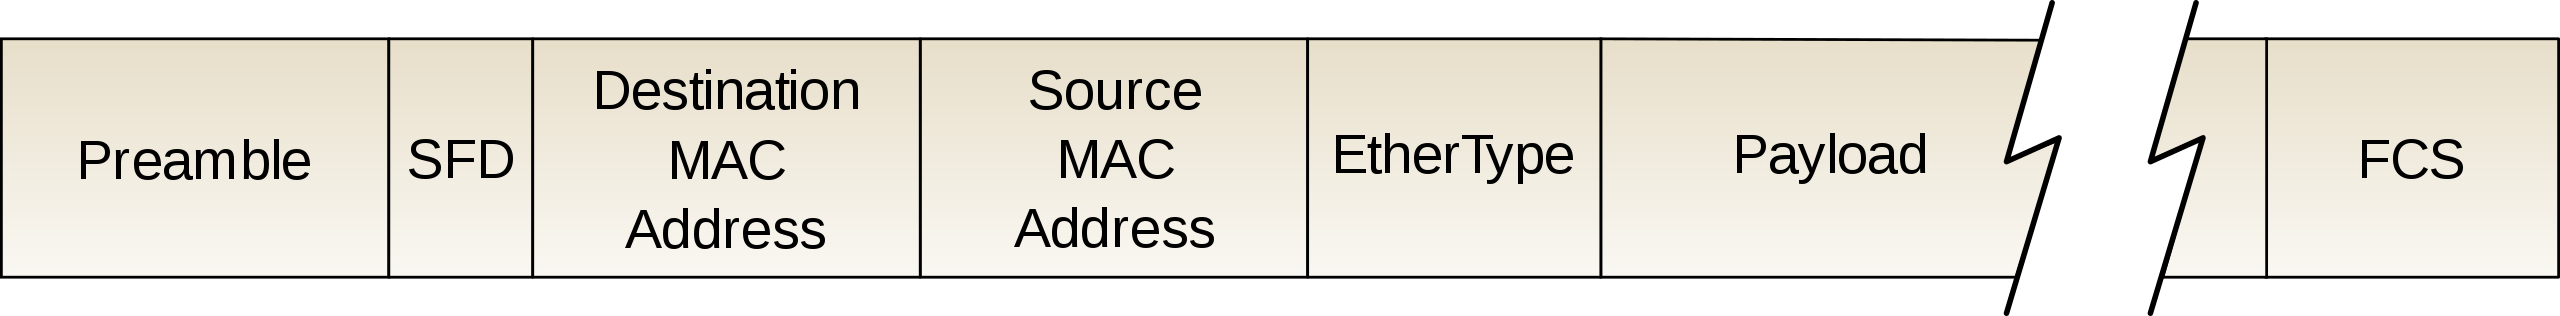
\includegraphics[width=\textwidth]{images/Ethernet_frame.png}
    \caption{An Ethernet frame inside an Ethernet packet, with SFD marking the end of the packet preamble and indicating the beginning of the frame}
    \label{fig:ethernet-frame}
\end{figure}


\Vref{fig:ethernet-frame} toont de velden in een Ethernet frame.
Eerst komen de \emph{preamble} en de \emph{start of frame delimiter} (SFD).
Deze dienen om het kloksignaal van de ontvanger af te stemmen op het kloksignaal van de zender zodat beide machines weten hoe lang het signaal van een 0 of een 1 duurt.

Hierna begint het eigenlijke Ethernet frame met het destination MAC-adres, gevolgd door het MAC-adres van de zender.
De \emph{EtherType} vertelt de ontvanger wat voor data er wordt verstuurd.
Enkele voorbeelden van geldige EtherTypes worden gegeven in \vref{tab:ethertype}.
Hierna komt de eigenlijke data of de \emph{payload} en ten slotte komt de \emph{frame check sequence} (FCS).
Dit is een code die gebruikt wordt om te detecteren of er fouten in het frame zitten.
Als het frame corrupt is, wordt deze gewoon verwijderd.
De ontvanger verwittigt de zender van het frame niet dat het frame niet goed is aangekomen.

\begin{table}[htp]
    \centering
    \begin{tabular}{ll}
    \textit{EtherType} & \textit{protocol} \\[1ex]
    0x0800 & IPv4 \\
    0x0806 & address resolution protocol (ARP) \\
    0x8100 & VLAN-tagged frame \\
    0x86DD & IPv6 \\
    \end{tabular}
    \caption{Enkele mogelijke waarden van de EtherType in een Ethernet frame}
    \label{tab:ethertype}
\end{table}


\section{Ethernetswitches}

Een Ethernetswitch ziet er niet anders uit dan een hub.
Een hub werkt echter heel anders dan een switch.
De interfaces van een hub zijn rechtstreeks met elkaar verbonden door middel van koperdraadjes zodat een elektrisch signaal dat binnenkomt op een van de interfaces, doorgestuurd wordt naar alle andere interfaces van de hub.
Een hub bevat geen intelligentie en kan niet geconfigureerd worden.

Een switch daarentegen is een toestel met heel wat intelligentie.
Er bestaan twee soorten switches: \emph{managed} en \emph{unmanaged} switches.
Unmanaged switches hebben de nodige intelligentie maar kunnen verder niet geconfigureerd worden.
Managed switches daarentegen beschikken over een volledig besturingssysteem en kunnen over zeer veel geavanceerde features beschikken.

\Vref{fig:ethernetswitch} toont een Juniper switch met 48~poorten of interfaces.
Rechts onder de display bevinden zich nog vier ``gaten'' in de switch.
Dit zijn sloten waar SFP-modules geplaatst kunnen worden (zie \vref{sec:sfp-modules}).

\begin{figure}
    \centering
    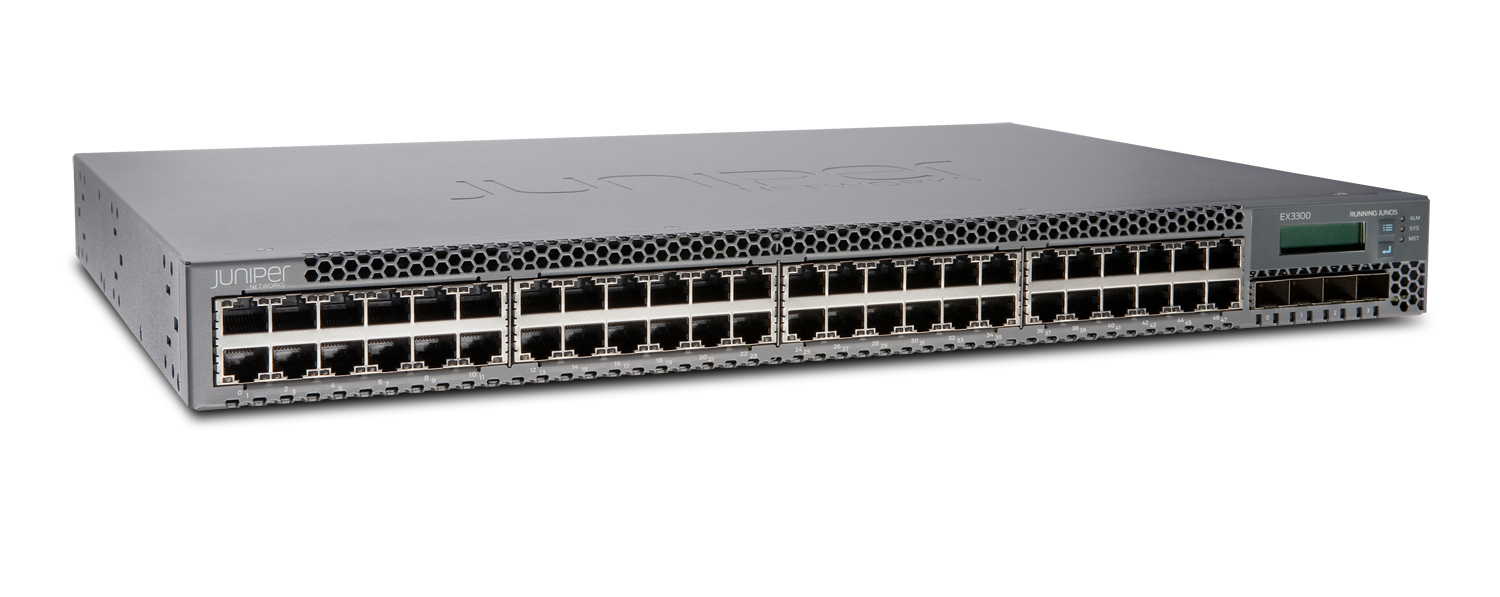
\includegraphics[width=\textwidth]{images/ethernetswitch.jpg}
    \caption{Een Ethernetswitch met 48 poorten en 4 openingen voor SFP-modules}
    \label{fig:ethernetswitch}
\end{figure}


In \vref{fig:simple-lan} zijn drie computers met elkaar verbonden via een switch.
Computer~1 wil communiceren met computer~2.
We gaan er even van uit dat beide computers elkaars IP-adres en MAC-adres kennen.
Als de switch de eerste frame ontvangt van computer~1, weet het nog niets over het netwerk of de toestellen die verbonden zijn met de switch, dus stuurt het het frame via alle interfaces naar buiten.
Computers~2 en~3 ontvangen dus dit eerste frame.
Computer~3 ziet het destination MAC-adres van het frame en, omdat dit niet zijn MAC-adres is, gooit het frame weg.
Computer~2 herkent wel zijn eigen MAC-adres in het frame en verwerkt de inhoud en stuurt uiteindelijk een antwoord terug.

De switch stuurt niet alleen het frame aan alle interfaces naar buiten, maar maakt ook notitie van het source MAC-adres en noteert dit in de MAC-tabel samen met de interface waarop hij het MAC-adres geleerd heeft.
\begin{center}
\begin{tabular}{cc}
\textit{MAC-adres} & \textit{interface} \\[1ex]
0200.aaaa.0001 & fa0/1\\
\end{tabular}
\end{center}
Als computer~2 nu een antwoord stuurt naar computer~1, komt dit frame aan op fa0/2 van de switch.
Weer noteert de switch het source MAC-adres in de MAC-tabel samen met de interface waarop de switch het frame ontvangt.
Vervolgens zoekt de switch het destination MAC-adres op in de MAC-tabel, vindt de bijhorende interface, en verstuurt het frame enkel langs deze interface naar buiten.
Computer~3 ziet dit antwoord -- en alle verder communicatie tussen computers~1 en~2 -- niet meer.

\begin{figure}
    \centering
    \documentclass[tikz]{standalone}
\usepackage{ifthen}
\usepackage{contour}
%%
%% Medtronic color palette
%%

\usepackage{xcolor}

% Primary blue color palette
\definecolor{mdtnavyblue}{cmyk}{1,.94,.47,.43}
\definecolor{mdtmedtronicblue}{cmyk}{.99,.74,.17,.04}
\definecolor{mdtcobaltblue}{cmyk}{.81,.35,0,0}
\definecolor{mdtmediumblue}{cmyk}{.73,.12,0,0}
\definecolor{mdtskyblue}{cmyk}{.55,.04,.04,0}
\definecolor{mdtlightblue}{cmyk}{.29,.05,.05,0}

% Primary neutral color palette
\definecolor{mdtcharcoal}{rgb}{.83,.86,.90}
\definecolor{mdtbluegray}{cmyk}{.68,.40,.28,.08}
\definecolor{mdtdarkgray}{cmyk}{0,0,0,.55}
\definecolor{mdtlightgray}{cmyk}{0,0,0,.30}
\definecolor{mdtpalegray}{cmyk}{.08,.06,.06,0}

% Accent colors
\definecolor{mdtyellow}{cmyk}{0,.18,.93,0}
\definecolor{mdtlightorange}{cmyk}{.02,.38,.96,0}
\definecolor{mdtorange}{cmyk}{.04,.78,1,0}
\definecolor{mdtpurple}{cmyk}{.38,.98,0,0}
\definecolor{mdtgreen}{cmyk}{.57,.02,1,0}
\definecolor{mdtturquoise}{cmyk}{.70,0,.38,0}

% TikZ/PGF
\usepackage{tikz}
\usetikzlibrary{backgrounds}
\usetikzlibrary{calc}
\usetikzlibrary{decorations.pathreplacing}
\usetikzlibrary{fit}
\usetikzlibrary{matrix}
\usetikzlibrary{patterns}
\usetikzlibrary{positioning}
\usetikzlibrary{shapes.geometric}
\usetikzlibrary{arrows}

%%
%% Styles
%%

% Network nodes
\tikzset{network node image/.style={
                inner sep=0mm,
                %anchor=south west
                }}
\tikzset{network node/.style={
                network node image,
                thick,
                text=mdtmedtronicblue,
                draw=mdtmedtronicblue,
                fill=white,
                minimum size=10mm}}
\tikzset{network node circle/.style={
                network node,
                circle}}
\tikzset{network node square/.style={
                network node,
                rectangle,
                rounded corners}}
\tikzset{network node rectangle/.style={
                network node,
                rectangle,
                minimum height=15mm,
                rounded corners}}
\tikzset{server rack/.style={
                align=left,
                text width=8mm,
                inner sep=0pt,
                anchor=north west,
                minimum height=7.5mm-.8pt,
                minimum width=10.7mm-.8pt,
                thick,
                text=mdtmedtronicblue,
                draw=mdtmedtronicblue,
                fill=white}}
\tikzset{network rack/.style={
                align=left,
                text width=9.3mm,
                inner sep=0pt,
                anchor=north west,
                minimum height=7.5mm-.8pt,
                minimum width=12mm-.8pt,
                %minimum height=7.5mm,
                %minimum width=12mm,
                thick,
                text=mdtmedtronicblue,
                draw=mdtmedtronicblue,
                fill=white}}
\tikzset{patch rack/.style={
                align=left,
                text width=9.3mm,
                inner sep=0pt,
                anchor=north west,
                minimum height=7.5mm-.8pt,
                minimum width=12mm-.8pt,
                thick,
                text=mdtmedtronicblue,
                draw=mdtmedtronicblue,
                fill=white}}

% Labels
\tikzset{interface label/.style={
                font=\footnotesize,
                inner sep=2pt},
                fill=white}
\tikzset{node label/.style={
                font=\small,
                align=center,
                inner sep=2pt,
                thick,
                rounded corners}}


% Floor tiles
\newcommand{\dcfloortiles}[2]{%
    \draw[step=6mm,gray,very thin] (0,0) grid ($.6*(#1,#2)$);
}
\newcommand{\dccoldaisle}[2]{%
    \draw[pattern=north west lines, pattern color=mdtlightgray] ($.6*(#1)-(.6,.6)$) rectangle ($.6*(#1)+.6*(#2)-(.6,.6)$);
}
% Markings for different types of racks
\newcommand{\caserack}[1]{%
    \draw[very thick,mdtorange] ($(#1.north east)-(.1,.1)$) -- ($(#1.south east)+(-.1,.1)$);
}
\newcommand{\storagerack}[1]{%
    \draw[very thick,mdtgreen] ($(#1.north east)-(.2,.1)$) -- ($(#1.south east)+(-.2,.1)$);
}
\newcommand{\networkrack}[1]{%
    \draw[very thick,mdtmediumblue] ($(#1.north east)-(.15,.1)$) -- ($(#1.south east)+(-.15,.1)$);
}
\newcommand{\mitgrack}[1]{%
    \draw[very thick,mdtpurple] ($(#1.north east)-(.25,.1)$) -- ($(#1.south east)+(-.25,.1)$);
}
\newcommand{\unixrack}[1]{%
    \draw[very thick,mdtdarkgray] ($(#1.north east)-(.3,.1)$) -- ($(#1.south east)+(-.3,.1)$);
}
\newcommand{\computerack}[1]{%
    \draw[very thick,mdtturquoise] ($(#1.north east)-(.35,.1)$) -- ($(#1.south east)+(-.35,.1)$);
}
\newcommand{\racklabels}[1]{%
    \matrix (racklabels) at (#1) [matrix of nodes,
        nodes={
            anchor=west,
            align=left
            }
        ] {
            |[mdtorange]| CASE \\
            |[mdtturquoise]| Compute (CORE) \\
            |[mdtpurple]| MITG \\
            |[mdtmediumblue]| Network \\
            |[mdtgreen]| Storage \\
            |[mdtdarkgray]| UNIX \\
    };
}
%
% layers.tex
%
% This document contains code to hide a PGF layer if so desired,
% e.g. you can hide the layer with all the labels on it.
%

% Define the layers to be used
\pgfdeclarelayer{connections}
\pgfdeclarelayer{interfaces}
\pgfdeclarelayer{hostnames}
\pgfdeclarelayer{labels}
\pgfdeclarelayer{arrows}

% Make the background white so we can hide the labels by swapping the order of the layers
\tikzset{show background rectangle,background rectangle/.style={rounded corners,fill=white}}

% \showalllayers - Show the nodes, connections, and detailed labels, including interface labels
% The left most layer is the bottom layer; everything left from the background will be hidden.
\newcommand\showalllayers{      \pgfsetlayers{hostnames,arrows,background,connections,main,interfaces,labels}}
\newcommand\showarrows{         \pgfsetlayers{hostnames,background,connections,main,interfaces,labels,arrows}}
% \hidelabels - Show only the nodes and the connections
\newcommand\hidelabels{         \pgfsetlayers{hostnames,arrows,interfaces,labels,background,connections,main}}
% \hideinterfaces - Hide only the interface labels
\newcommand\hideinterfaces{     \pgfsetlayers{hostnames,arrows,interfaces,background,connections,main,labels}}
% \showonlyhostnames - Hide everything but show the hostnames only
\newcommand\showonlyhostnames{  \pgfsetlayers{arrows,interfaces,labels,background,connections,main,hostnames}}
\newcommand\showhostnamesinterfaces{ \pgfsetlayers{arrows,labels,background,connections,main,hostnames,interfaces}}
% Default setting is to show all layers
\showalllayers
%
% connections.tex
%
% This document contains all the commands needed to create connections between
% different network nodes, e.g.
%  - a normal connection, with our without labels.
%  - a vPC connection between 3 or 4 nodes.
%

%
% Syntax:
% \connect[<color>]{<node1>}{<intf1>}{<node2>}{<intf2>}
\newcommand{\connect}[5][black]{

    % Save the coordinates for the interface labels
    \path (#2) -- (#4) coordinate[very near start] (i1) coordinate[midway] (im) coordinate[very near end] (i2);
    
    % Draw the connection between the two devices on the correct layer.
    \begin{pgfonlayer}{connections}
      \draw[color=#1] (#2) -- (#4);
    \end{pgfonlayer}
    
    % Draw the interface labels on the correct layer.
    \begin{pgfonlayer}{interfaces}
        \ifthenelse{\equal{#3}{}}{}{\node[interface label,fill=white] at (i1) {\contour{white}{#3}};}
        \ifthenelse{\equal{#5}{}}{}{\node[interface label,fill=white] at (i2) {\contour{white}{#5}};}
    \end{pgfonlayer}
    
    %\ifthenelse{\equal{#5}{}}{
    %    % Parameter 5 is empty:
    %    \ifthenelse{\equal{#3}{}}{
    %        % Parameter 3 is empty: no interfaces have been given.
    %        \draw[color=#1] (#2) -- (#4);
    %    }{
    %        % Both devices share the same interface name.
    %        \draw[color=#1] (#2) -- (#4)
    %            node [midway,interface] {#3};
    %    }
    %}{
    %    % Parameter 5 is not empty: both interfaces are given.
    %    \draw[color=#1] (#2) -- (#4)
    %        node [on background layer,near start,interface] {#3}
    %        node [near end,interface] {#5};
    %}
}

%
% Syntax:
% \connectClusters[<straight/cross>]{cluster1}{cluster2}
\newcommand{\connectClusters}[3][S]{
    \message{connectClusters 2-1: #2-1^^J}
    \message{connectClusters 2-2: #2-2^^J}
    \message{connectClusters 3-1: #3-1^^J}
    \message{connectClusters 3-2: #3-2^^J}
    \ifthenelse{\equal{#1}{S}}{
        \connect{#2-1}{}{#3-1}{}
        \connect{#2-2}{}{#3-2}{}
    }{
        \connect{#2-1}{}{#3-2}{}
        \connect{#2-2}{}{#3-1}{}
    }
}

%
% Syntax:
% \arrowcoords[<position>]{<coordinates start>}{<coordinates end>}{<text>}
\newcommand{\arrowcoords}[4][midway]{
    \draw[mdtgreen, arrows={-latex'}, shorten <= 0.25cm, shorten >= 0.25cm, very thick, distance=2cm] (#2) to[out=230,in=170] (#3) node[#1] {#4};
}

%
%
%

\def\iconset{3015}


%
% Display only the icons
%
% Syntax: \icon<type>{<hostname>}{<coordinates>}
%

\newcommand{\iconcloud}[2]{
    \node[network node image] (#1) at (#2) {
\includegraphics[width=30mm]{images//cloud.png}};
    \node at ([yshift=-2mm]#2) {#1};
}
\newcommand{\iconfirewall}[2]{
    \ifthenelse{\equal{\iconset}{basic}}{
        \node[network node circle,draw=mdtorange] (#1) at (#2) {FW};
    }{
        \node[network node image] (#1) at (#2) {
\includegraphics[width=10mm]{images/\iconset/firewall.eps}};
    }
}
\newcommand{\iconips}[2]{
    \ifthenelse{\equal{\iconset}{basic}}{
        \node[network node square] (#1) at (#2) {IPS};
    }{
        \node[network node image] (#1) at (#2) {\includegraphics[width=10mm]{images/\iconset/ips.eps}};
    }
}
\newcommand{\iconrouter}[2]{
    \ifthenelse{\equal{\iconset}{basic}}{
        \node[network node circle] (#1) at (#2) {RTR};
    }{
        \node[network node image] (#1) at (#2) {
\includegraphics[width=10mm]{images/\iconset/router.eps}};
    }
    \message{iconrouter: #1^^J}
}
\newcommand{\iconswitch}[2]{
    \ifthenelse{\equal{\iconset}{basic}}{
        \node[network node square] (#1) at (#2) {SW};
    }{
        \node[network node image] (#1) at (#2) {
\includegraphics[width=13mm]{images/\iconset/switch.eps}};
    }
}
\newcommand{\icondistswitch}[2]{
    \ifthenelse{\equal{\iconset}{basic}}{
        \node[network node square] (#1) at (#2) {SW};
    }{
        \node[network node image] (#1) at (#2) {\includegraphics[width=13mm]{images/\iconset/l3switch.eps}};
    }
}
\newcommand{\iconcoreswitch}[2]{
    \ifthenelse{\equal{\iconset}{basic}}{
        \node[network node square] (#1) at (#2) {SW};
    }{
        \node[network node image] (#1) at (#2) {\includegraphics[width=13mm]{images/\iconset/coreswitch.eps}};
    }
}
\newcommand{\iconhost}[2]{
   \ifthenelse{\equal{\iconset}{basic}}{
      \node[network node square] (#1) at (#2) {PC};
   }{
      \node[network node square] (#1) at (#2) {PC};
   }
}



%
% Display the node: icon + labels
%
%
% Syntax: \node<type>[<label position>]{<name>}{<coordinates>}{<type>}{<IP address>}
%
% Where:
%  - <label position> : top, bottom, left, right (default)
%  - <type> : hardware type, e.g. Catalyst 3850
%

\newcommand{\nodecloud}[5][right]{
    \iconcloud{#2}{#3}
}
\newcommand{\nodefirewall}[5][right]{
    \iconfirewall{#2}{#3}
    \nodelabel[#1]{#3}{#2}{#4}{#5}
}
\newcommand{\nodeips}[5][right]{
    \iconips{#2}{#3}
    \nodelabel[#1]{#3}{#2}{#4}{#5}
}
\newcommand{\noderouter}[5][right]{
    \iconrouter{#2}{#3}
    \nodelabel[#1]{#3}{#2}{#4}{#5}
}
\newcommand{\nodedistswitch}[5][right]{
    \icondistswitch{#2}{#3}
    \nodelabel[#1]{#3}{#2}{#4}{#5}
}
\newcommand{\nodeswitch}[5][right]{    
    \iconswitch{#2}{#3}
    \nodelabel[#1]{#3}{#2}{#4}{#5}
}
\newcommand{\nodecoreswitch}[5][right]{    
    \iconcoreswitch{#2}{#3}
    \nodelabel[#1]{$(#3)-(0,.4)$}{#2}{#4}{#5}
}
\newcommand{\nodehost}[5][right]{
   \iconhost{#2}{#3}
   \nodelabel[#1]{#3}{#2}{#4}{#5}
}



%
% Clusters of nodes
%
% Syntax: \cluster<type>[<label position>]{<name>}{<coordinates>}{<type>}{<IP address>}
%

\newcommand{\clustercloud}[3][bottom]{
    \draw[network node,draw=mdtpurple,fill=mdtpalegray] (#3) ellipse (15mm and 10mm);
    \node (#2) at (#3) {#2};
    \ifthenelse{\equal{#1}{top}}{
        \coordinate (a) at ($(#3)-(10mm,-7mm)$);
        \coordinate (b) at ($(#3)+(10mm,7mm)$);
    }{
        \coordinate (a) at ($(#3)-(10mm,7mm)$);
        \coordinate (b) at ($(#3)+(10mm,-7mm)$);
    }
    \message{clustercloud: #2-1^^J}
    \iconrouter{#2-1}{a}
    \message{clustercloud: #2-2^^J}
    \iconrouter{#2-2}{b}
}

\newcommand{\clusterfirewall}[5][bottom]{
    \coordinate (left) at ($(#3)-(1,0)$);
    \coordinate (right) at ($(#3)+(1,0)$);
    \iconfirewall{#2-1}{left}
    \iconfirewall{#2-2}{right}
    
    \begin{pgfonlayer}{connections}
        \node (#2) [draw=mdtmedtronicblue,rounded corners,inner sep=2mm,dashed,fit=(#2-1) (#2-2)] {};
    \end{pgfonlayer}
    \connect{#2-1}{}{#2-2}{}
    
    \nodelabel[#1]{#3}{#2}{#4}{#5}
}




%
% Syntax:
% \nodelabel[<position>]{<coordinates>}{<hostname>}{<type>}{<IP address>}
\newcommand{\nodelabel}[5][right]{
    \def\text{\contour{white}{\textbf{#3}}\\\contour{white}{\emph{#4}}\\\contour{white}{#5}}
    \begin{pgfonlayer}{labels}
    
    % On the right
    \ifthenelse{\equal{#1}{right}}{
        %\node[node label,anchor=west] at ($(#2)+(1,0)$) {\contour{white}{\textbf{#3}\\\emph{#4}\\#5}};
        \node[node label,anchor=west] at ($(#2)+(1,0)$) {\text};
        
    % On the left
    }{\ifthenelse{\equal{#1}{left}}{
        \node[node label,anchor=east] at ($(#2)-(1,0)$) {\text};
    
    % At the top
    }{\ifthenelse{\equal{#1}{top}}{
        \node[node label,anchor=south] at ($(#2)+(0,1)$) {\text};
    
    % At the bottom
    }{\ifthenelse{\equal{#1}{bottom}}{
        \node[node label,anchor=north] at ($(#2)-(0,1)$) {\text};
    
    }{}}}}
    
    \end{pgfonlayer}
    
    \begin{pgfonlayer}{hostnames}
        \node[node label,anchor=north] at ($(#2)-(0,.6)$) {\contour{white}{#3}};
    \end{pgfonlayer}
}

%
% Syntax:
% \vlaninformationR[<xshift>]{<node name>}{<relative location>}
%\newcommand{\vlaninformationR}[4][5cm]{
%    \matrix (#2) [matrix of nodes,
%        right=of #3,
%        xshift=#1,
%        left delimiter=\{,
%        nodes={
%            anchor=west,
%            align=left
%            }
%        ] {
%            #4
%    };
%}
\begin{document}
\begin{tikzpicture}[framed]
\def\iconset{basic}
%\showhostnamesinterfaces
\nodeswitch[bottom]{switch}{3,0}{Cisco 2960}{}
\nodehost[left]{pc 1}{0,0}{FreeBSD}{0200.aaaa.0001}
\nodehost{pc 2}{6,0}{FreeBSD}{0200.aaaa.0002}
\nodehost{pc 3}{3,3}{Linux}{0200.aaaa.0003}
\connect{switch}{fa0/1}{pc 1}{em0}
\connect{switch}{fa0/2}{pc 2}{em0}
\connect{switch}{fa0/3}{pc 3}{eth0}


\end{tikzpicture}
\end{document}
    \caption{Een eenvoudig netwerk met twee computers die met elkaar verbonden zijn via een switch}
    \label{fig:simple-lan}
\end{figure}

Een MAC-adres kan slechts aan één interface gekoppeld zijn.
Als de switch een MAC-adres dat het al kent, opnieuw leert via een andere interface, dan update het de bestaande entry in de MAC-tabel door de oude interface te vervangen door de nieuwe interface.

Het is wel mogelijk dat meerdere MAC-adressen op dezelfde interface geleerd worden.
Dit is mogelijk als een computer met meerdere virtuele machines, verbonden wordt met de switch.
Elke virtuele machine heeft immers een eigen MAC-adres.
Het is ook mogelijk meerdere MAC-adressen te leren op een interface als deze interface met een andere switch verbindt.
De eerste switch leert dan de MAC-adressen van alle computers die verbinden met de tweede switch via deze interface.


\section{Lussen in het netwerk}
\label{sec:stp}

Als één switch niet meer voldoende is om alle computers en printers met elkaar te verbinden, verbinden we een tweede switch met de eerste switch.
Als beide switch niet meer voldoende zijn, kunnen we nog een derde switch verbinden met het netwerk, en vervolgens nog een vierde en vijfde switch (zie \vref{fig:daisy-chain}).
Een dergelijk netwerk kan lang goed functioneren.
Tot op een dag bijvoorbeeld switch~2 kapot gaat en alle computers die met switches~3 tot en met~5 verbonden zijn, geen Internetconnectiviteit meer hebben.
Maar dit is eenvoudig op te lossen.
We verbinden switch~1 snel met switch~3 en de connectiviteit is hersteld.


\begin{figure}
    \centering
    \documentclass[tikz]{standalone}
\usepackage{ifthen}
\usepackage{contour}
%%
%% Medtronic color palette
%%

\usepackage{xcolor}

% Primary blue color palette
\definecolor{mdtnavyblue}{cmyk}{1,.94,.47,.43}
\definecolor{mdtmedtronicblue}{cmyk}{.99,.74,.17,.04}
\definecolor{mdtcobaltblue}{cmyk}{.81,.35,0,0}
\definecolor{mdtmediumblue}{cmyk}{.73,.12,0,0}
\definecolor{mdtskyblue}{cmyk}{.55,.04,.04,0}
\definecolor{mdtlightblue}{cmyk}{.29,.05,.05,0}

% Primary neutral color palette
\definecolor{mdtcharcoal}{rgb}{.83,.86,.90}
\definecolor{mdtbluegray}{cmyk}{.68,.40,.28,.08}
\definecolor{mdtdarkgray}{cmyk}{0,0,0,.55}
\definecolor{mdtlightgray}{cmyk}{0,0,0,.30}
\definecolor{mdtpalegray}{cmyk}{.08,.06,.06,0}

% Accent colors
\definecolor{mdtyellow}{cmyk}{0,.18,.93,0}
\definecolor{mdtlightorange}{cmyk}{.02,.38,.96,0}
\definecolor{mdtorange}{cmyk}{.04,.78,1,0}
\definecolor{mdtpurple}{cmyk}{.38,.98,0,0}
\definecolor{mdtgreen}{cmyk}{.57,.02,1,0}
\definecolor{mdtturquoise}{cmyk}{.70,0,.38,0}

% TikZ/PGF
\usepackage{tikz}
\usetikzlibrary{backgrounds}
\usetikzlibrary{calc}
\usetikzlibrary{decorations.pathreplacing}
\usetikzlibrary{fit}
\usetikzlibrary{matrix}
\usetikzlibrary{patterns}
\usetikzlibrary{positioning}
\usetikzlibrary{shapes.geometric}
\usetikzlibrary{arrows}

%%
%% Styles
%%

% Network nodes
\tikzset{network node image/.style={
                inner sep=0mm,
                %anchor=south west
                }}
\tikzset{network node/.style={
                network node image,
                thick,
                text=mdtmedtronicblue,
                draw=mdtmedtronicblue,
                fill=white,
                minimum size=10mm}}
\tikzset{network node circle/.style={
                network node,
                circle}}
\tikzset{network node square/.style={
                network node,
                rectangle,
                rounded corners}}
\tikzset{network node rectangle/.style={
                network node,
                rectangle,
                minimum height=15mm,
                rounded corners}}
\tikzset{server rack/.style={
                align=left,
                text width=8mm,
                inner sep=0pt,
                anchor=north west,
                minimum height=7.5mm-.8pt,
                minimum width=10.7mm-.8pt,
                thick,
                text=mdtmedtronicblue,
                draw=mdtmedtronicblue,
                fill=white}}
\tikzset{network rack/.style={
                align=left,
                text width=9.3mm,
                inner sep=0pt,
                anchor=north west,
                minimum height=7.5mm-.8pt,
                minimum width=12mm-.8pt,
                %minimum height=7.5mm,
                %minimum width=12mm,
                thick,
                text=mdtmedtronicblue,
                draw=mdtmedtronicblue,
                fill=white}}
\tikzset{patch rack/.style={
                align=left,
                text width=9.3mm,
                inner sep=0pt,
                anchor=north west,
                minimum height=7.5mm-.8pt,
                minimum width=12mm-.8pt,
                thick,
                text=mdtmedtronicblue,
                draw=mdtmedtronicblue,
                fill=white}}

% Labels
\tikzset{interface label/.style={
                font=\footnotesize,
                inner sep=2pt},
                fill=white}
\tikzset{node label/.style={
                font=\small,
                align=center,
                inner sep=2pt,
                thick,
                rounded corners}}


% Floor tiles
\newcommand{\dcfloortiles}[2]{%
    \draw[step=6mm,gray,very thin] (0,0) grid ($.6*(#1,#2)$);
}
\newcommand{\dccoldaisle}[2]{%
    \draw[pattern=north west lines, pattern color=mdtlightgray] ($.6*(#1)-(.6,.6)$) rectangle ($.6*(#1)+.6*(#2)-(.6,.6)$);
}
% Markings for different types of racks
\newcommand{\caserack}[1]{%
    \draw[very thick,mdtorange] ($(#1.north east)-(.1,.1)$) -- ($(#1.south east)+(-.1,.1)$);
}
\newcommand{\storagerack}[1]{%
    \draw[very thick,mdtgreen] ($(#1.north east)-(.2,.1)$) -- ($(#1.south east)+(-.2,.1)$);
}
\newcommand{\networkrack}[1]{%
    \draw[very thick,mdtmediumblue] ($(#1.north east)-(.15,.1)$) -- ($(#1.south east)+(-.15,.1)$);
}
\newcommand{\mitgrack}[1]{%
    \draw[very thick,mdtpurple] ($(#1.north east)-(.25,.1)$) -- ($(#1.south east)+(-.25,.1)$);
}
\newcommand{\unixrack}[1]{%
    \draw[very thick,mdtdarkgray] ($(#1.north east)-(.3,.1)$) -- ($(#1.south east)+(-.3,.1)$);
}
\newcommand{\computerack}[1]{%
    \draw[very thick,mdtturquoise] ($(#1.north east)-(.35,.1)$) -- ($(#1.south east)+(-.35,.1)$);
}
\newcommand{\racklabels}[1]{%
    \matrix (racklabels) at (#1) [matrix of nodes,
        nodes={
            anchor=west,
            align=left
            }
        ] {
            |[mdtorange]| CASE \\
            |[mdtturquoise]| Compute (CORE) \\
            |[mdtpurple]| MITG \\
            |[mdtmediumblue]| Network \\
            |[mdtgreen]| Storage \\
            |[mdtdarkgray]| UNIX \\
    };
}
%
% layers.tex
%
% This document contains code to hide a PGF layer if so desired,
% e.g. you can hide the layer with all the labels on it.
%

% Define the layers to be used
\pgfdeclarelayer{connections}
\pgfdeclarelayer{interfaces}
\pgfdeclarelayer{hostnames}
\pgfdeclarelayer{labels}
\pgfdeclarelayer{arrows}

% Make the background white so we can hide the labels by swapping the order of the layers
\tikzset{show background rectangle,background rectangle/.style={rounded corners,fill=white}}

% \showalllayers - Show the nodes, connections, and detailed labels, including interface labels
% The left most layer is the bottom layer; everything left from the background will be hidden.
\newcommand\showalllayers{      \pgfsetlayers{hostnames,arrows,background,connections,main,interfaces,labels}}
\newcommand\showarrows{         \pgfsetlayers{hostnames,background,connections,main,interfaces,labels,arrows}}
% \hidelabels - Show only the nodes and the connections
\newcommand\hidelabels{         \pgfsetlayers{hostnames,arrows,interfaces,labels,background,connections,main}}
% \hideinterfaces - Hide only the interface labels
\newcommand\hideinterfaces{     \pgfsetlayers{hostnames,arrows,interfaces,background,connections,main,labels}}
% \showonlyhostnames - Hide everything but show the hostnames only
\newcommand\showonlyhostnames{  \pgfsetlayers{arrows,interfaces,labels,background,connections,main,hostnames}}
\newcommand\showhostnamesinterfaces{ \pgfsetlayers{arrows,labels,background,connections,main,hostnames,interfaces}}
% Default setting is to show all layers
\showalllayers
%
% connections.tex
%
% This document contains all the commands needed to create connections between
% different network nodes, e.g.
%  - a normal connection, with our without labels.
%  - a vPC connection between 3 or 4 nodes.
%

%
% Syntax:
% \connect[<color>]{<node1>}{<intf1>}{<node2>}{<intf2>}
\newcommand{\connect}[5][black]{

    % Save the coordinates for the interface labels
    \path (#2) -- (#4) coordinate[very near start] (i1) coordinate[midway] (im) coordinate[very near end] (i2);
    
    % Draw the connection between the two devices on the correct layer.
    \begin{pgfonlayer}{connections}
      \draw[color=#1] (#2) -- (#4);
    \end{pgfonlayer}
    
    % Draw the interface labels on the correct layer.
    \begin{pgfonlayer}{interfaces}
        \ifthenelse{\equal{#3}{}}{}{\node[interface label,fill=white] at (i1) {\contour{white}{#3}};}
        \ifthenelse{\equal{#5}{}}{}{\node[interface label,fill=white] at (i2) {\contour{white}{#5}};}
    \end{pgfonlayer}
    
    %\ifthenelse{\equal{#5}{}}{
    %    % Parameter 5 is empty:
    %    \ifthenelse{\equal{#3}{}}{
    %        % Parameter 3 is empty: no interfaces have been given.
    %        \draw[color=#1] (#2) -- (#4);
    %    }{
    %        % Both devices share the same interface name.
    %        \draw[color=#1] (#2) -- (#4)
    %            node [midway,interface] {#3};
    %    }
    %}{
    %    % Parameter 5 is not empty: both interfaces are given.
    %    \draw[color=#1] (#2) -- (#4)
    %        node [on background layer,near start,interface] {#3}
    %        node [near end,interface] {#5};
    %}
}

%
% Syntax:
% \connectClusters[<straight/cross>]{cluster1}{cluster2}
\newcommand{\connectClusters}[3][S]{
    \message{connectClusters 2-1: #2-1^^J}
    \message{connectClusters 2-2: #2-2^^J}
    \message{connectClusters 3-1: #3-1^^J}
    \message{connectClusters 3-2: #3-2^^J}
    \ifthenelse{\equal{#1}{S}}{
        \connect{#2-1}{}{#3-1}{}
        \connect{#2-2}{}{#3-2}{}
    }{
        \connect{#2-1}{}{#3-2}{}
        \connect{#2-2}{}{#3-1}{}
    }
}

%
% Syntax:
% \arrowcoords[<position>]{<coordinates start>}{<coordinates end>}{<text>}
\newcommand{\arrowcoords}[4][midway]{
    \draw[mdtgreen, arrows={-latex'}, shorten <= 0.25cm, shorten >= 0.25cm, very thick, distance=2cm] (#2) to[out=230,in=170] (#3) node[#1] {#4};
}

%
%
%

\def\iconset{3015}


%
% Display only the icons
%
% Syntax: \icon<type>{<hostname>}{<coordinates>}
%

\newcommand{\iconcloud}[2]{
    \node[network node image] (#1) at (#2) {
\includegraphics[width=30mm]{images//cloud.png}};
    \node at ([yshift=-2mm]#2) {#1};
}
\newcommand{\iconfirewall}[2]{
    \ifthenelse{\equal{\iconset}{basic}}{
        \node[network node circle,draw=mdtorange] (#1) at (#2) {FW};
    }{
        \node[network node image] (#1) at (#2) {
\includegraphics[width=10mm]{images/\iconset/firewall.eps}};
    }
}
\newcommand{\iconips}[2]{
    \ifthenelse{\equal{\iconset}{basic}}{
        \node[network node square] (#1) at (#2) {IPS};
    }{
        \node[network node image] (#1) at (#2) {\includegraphics[width=10mm]{images/\iconset/ips.eps}};
    }
}
\newcommand{\iconrouter}[2]{
    \ifthenelse{\equal{\iconset}{basic}}{
        \node[network node circle] (#1) at (#2) {RTR};
    }{
        \node[network node image] (#1) at (#2) {
\includegraphics[width=10mm]{images/\iconset/router.eps}};
    }
    \message{iconrouter: #1^^J}
}
\newcommand{\iconswitch}[2]{
    \ifthenelse{\equal{\iconset}{basic}}{
        \node[network node square] (#1) at (#2) {SW};
    }{
        \node[network node image] (#1) at (#2) {
\includegraphics[width=13mm]{images/\iconset/switch.eps}};
    }
}
\newcommand{\icondistswitch}[2]{
    \ifthenelse{\equal{\iconset}{basic}}{
        \node[network node square] (#1) at (#2) {SW};
    }{
        \node[network node image] (#1) at (#2) {\includegraphics[width=13mm]{images/\iconset/l3switch.eps}};
    }
}
\newcommand{\iconcoreswitch}[2]{
    \ifthenelse{\equal{\iconset}{basic}}{
        \node[network node square] (#1) at (#2) {SW};
    }{
        \node[network node image] (#1) at (#2) {\includegraphics[width=13mm]{images/\iconset/coreswitch.eps}};
    }
}
\newcommand{\iconhost}[2]{
   \ifthenelse{\equal{\iconset}{basic}}{
      \node[network node square] (#1) at (#2) {PC};
   }{
      \node[network node square] (#1) at (#2) {PC};
   }
}



%
% Display the node: icon + labels
%
%
% Syntax: \node<type>[<label position>]{<name>}{<coordinates>}{<type>}{<IP address>}
%
% Where:
%  - <label position> : top, bottom, left, right (default)
%  - <type> : hardware type, e.g. Catalyst 3850
%

\newcommand{\nodecloud}[5][right]{
    \iconcloud{#2}{#3}
}
\newcommand{\nodefirewall}[5][right]{
    \iconfirewall{#2}{#3}
    \nodelabel[#1]{#3}{#2}{#4}{#5}
}
\newcommand{\nodeips}[5][right]{
    \iconips{#2}{#3}
    \nodelabel[#1]{#3}{#2}{#4}{#5}
}
\newcommand{\noderouter}[5][right]{
    \iconrouter{#2}{#3}
    \nodelabel[#1]{#3}{#2}{#4}{#5}
}
\newcommand{\nodedistswitch}[5][right]{
    \icondistswitch{#2}{#3}
    \nodelabel[#1]{#3}{#2}{#4}{#5}
}
\newcommand{\nodeswitch}[5][right]{    
    \iconswitch{#2}{#3}
    \nodelabel[#1]{#3}{#2}{#4}{#5}
}
\newcommand{\nodecoreswitch}[5][right]{    
    \iconcoreswitch{#2}{#3}
    \nodelabel[#1]{$(#3)-(0,.4)$}{#2}{#4}{#5}
}
\newcommand{\nodehost}[5][right]{
   \iconhost{#2}{#3}
   \nodelabel[#1]{#3}{#2}{#4}{#5}
}



%
% Clusters of nodes
%
% Syntax: \cluster<type>[<label position>]{<name>}{<coordinates>}{<type>}{<IP address>}
%

\newcommand{\clustercloud}[3][bottom]{
    \draw[network node,draw=mdtpurple,fill=mdtpalegray] (#3) ellipse (15mm and 10mm);
    \node (#2) at (#3) {#2};
    \ifthenelse{\equal{#1}{top}}{
        \coordinate (a) at ($(#3)-(10mm,-7mm)$);
        \coordinate (b) at ($(#3)+(10mm,7mm)$);
    }{
        \coordinate (a) at ($(#3)-(10mm,7mm)$);
        \coordinate (b) at ($(#3)+(10mm,-7mm)$);
    }
    \message{clustercloud: #2-1^^J}
    \iconrouter{#2-1}{a}
    \message{clustercloud: #2-2^^J}
    \iconrouter{#2-2}{b}
}

\newcommand{\clusterfirewall}[5][bottom]{
    \coordinate (left) at ($(#3)-(1,0)$);
    \coordinate (right) at ($(#3)+(1,0)$);
    \iconfirewall{#2-1}{left}
    \iconfirewall{#2-2}{right}
    
    \begin{pgfonlayer}{connections}
        \node (#2) [draw=mdtmedtronicblue,rounded corners,inner sep=2mm,dashed,fit=(#2-1) (#2-2)] {};
    \end{pgfonlayer}
    \connect{#2-1}{}{#2-2}{}
    
    \nodelabel[#1]{#3}{#2}{#4}{#5}
}




%
% Syntax:
% \nodelabel[<position>]{<coordinates>}{<hostname>}{<type>}{<IP address>}
\newcommand{\nodelabel}[5][right]{
    \def\text{\contour{white}{\textbf{#3}}\\\contour{white}{\emph{#4}}\\\contour{white}{#5}}
    \begin{pgfonlayer}{labels}
    
    % On the right
    \ifthenelse{\equal{#1}{right}}{
        %\node[node label,anchor=west] at ($(#2)+(1,0)$) {\contour{white}{\textbf{#3}\\\emph{#4}\\#5}};
        \node[node label,anchor=west] at ($(#2)+(1,0)$) {\text};
        
    % On the left
    }{\ifthenelse{\equal{#1}{left}}{
        \node[node label,anchor=east] at ($(#2)-(1,0)$) {\text};
    
    % At the top
    }{\ifthenelse{\equal{#1}{top}}{
        \node[node label,anchor=south] at ($(#2)+(0,1)$) {\text};
    
    % At the bottom
    }{\ifthenelse{\equal{#1}{bottom}}{
        \node[node label,anchor=north] at ($(#2)-(0,1)$) {\text};
    
    }{}}}}
    
    \end{pgfonlayer}
    
    \begin{pgfonlayer}{hostnames}
        \node[node label,anchor=north] at ($(#2)-(0,.6)$) {\contour{white}{#3}};
    \end{pgfonlayer}
}

%
% Syntax:
% \vlaninformationR[<xshift>]{<node name>}{<relative location>}
%\newcommand{\vlaninformationR}[4][5cm]{
%    \matrix (#2) [matrix of nodes,
%        right=of #3,
%        xshift=#1,
%        left delimiter=\{,
%        nodes={
%            anchor=west,
%            align=left
%            }
%        ] {
%            #4
%    };
%}
\begin{document}
\begin{tikzpicture}[framed]
\def\iconset{basic}
\nodecloud{Internet}{0,4}{}{}
\nodefirewall{firewall}{0,2}{}{}
\nodeswitch[bottom]{sw1}{0,0}{}{}
\nodeswitch[bottom]{sw2}{2,0}{}{}
\nodeswitch[bottom]{sw3}{4,0}{}{}
\nodeswitch[bottom]{sw4}{6,0}{}{}
\nodeswitch[bottom]{sw5}{8,0}{}{}
\connect{Internet}{}{firewall}{}
\connect{firewall}{}{sw1}{}
\connect{sw1}{}{sw2}{}
\connect{sw2}{}{sw3}{}
\connect{sw3}{}{sw4}{}
\connect{sw4}{}{sw5}{}
\end{tikzpicture}
\end{document}
    \caption{Meerdere switches worden met elkaar verbonden in een lange lijn. Dit noemt \emph{daisy chaining}.}
    \label{fig:daisy-chain}
\end{figure}


Dit brengt echter een groot gevaar met zich mee.
Zolang switch~2 defect blijft, is er niets aan de hand.
Maar zodra switch~2 vervangen wordt door een nieuwe switch, hebben we een lus gemaakt in het netwerk.
Switch~1 verbindt met switch~2, zo met switch~3 en dan opnieuw naar switch~1.
Dit lijkt onschadelijk maar is dat zeker niet.

Neem opnieuw een computer verbonden met switch~1.
Deze wil met een andere computer in het netwerk communiceren.
De MAC-tabellen van alle drie de switches zijn leeg.
Als het eerste frame van de computer aankomt op switch~1, kan deze het source MAC-adres invullen zijn MAC-tabel maar omdat hij het destination MAC-adres niet kent, stuurt hij het frame via alle interfaces naar buiten.
Dit frame komt dus zowel bij switch~2 als bij switch~3 aan.
Switch~2 heeft ook een lege MAC-tabel dus stuurt het frame ook aan alle interfaces naar buiten, dus ook naar switch~3.

Switch~3 ontvangt het frame dus twee keer, een keer van switch~1 en een keer van switch~2.
Omdat het destination MAC-adres nog altijd niet bekend is, stuurt de switch beide frames langs alle interfaces naar buiten.
Switch~3 stuurt het frame dat hij van switch~2 gekregen heeft, door naar switch~1 en stuurt het frame van switch~1 door naar switch~2.

Eén frame heeft zich via deze lus verdubbeld en deze twee frames blijven rondlussen in het netwerk.
Dit soort fysieke lussen in het netwerk, kunnen een netwerk snel op de knieën brengen.



\section{Spanning-tree protocol (STP)}
Deze fysieke lussen zijn goed.
Als een switch of kabel kapot gaat, hebben de computers nog steeds netwerkconnectiviteit via de andere route.
Maar door de manier waarop switches omgaan met BUM-verkeer (broadcast, unknown unicast, multicast -- voor deze drie types heeft een switch nooit het destination MAC-adres in de MAC-tabel) zijn deze fysieke lussen net schadelijk voor je netwerk.
Het \emph{spanning-tree protocol} (STP) is een protocol dat deze fysieke lussen detecteert en telkens één interface in de lus uitschakelt.
Op die manier is het gevaar geweken want de frames kunnen niet meer eindelijk rondjes blijven draaien in de lus.
Als er echter een switch of kabel kapot gaat, wordt dit gedetecteerd door STP en wordt de interface die werd uitgezet, terug aangezet.

Spanning-tree protocol doet dit met behulp van \emph{bridge protocol data units} (BPDU),%
    \footnote{%
        De term ``bridge'' is een oude term voor ``switch.''
        Er waren enkele technische verschillen tussen beide soorten toestellen maar nu kunnen beide termen door elkaar gebruikt worden.%
        In de technische documentatie rondom STP wordt nog steeds bijna uitsluitend de term ``bridge'' gebruikt.
    }
speciale frames die switches naar elkaar sturen om informatie uit te wisselen over de status van het netwerk.
STP doorloopt vier stappen om een \emph{loop-free network} te bekomen.
\begin{enumerate}
\item
    Beslis samen welke switch de \emph{root bridge} wordt van het netwerk.
    Deze switch is als het ware de baas en verstuurt de BPDU's waarop de andere switches hun keuzes baseren.
    We kunnen de root bridge ook zien als de stam van de boom waar alle andere switches en verbindingen van aftakken.
\item
    Elke switch bepaalt de kortste route naar de root bridge en markeert deze interface als de \emph{root port}.
\item
    Elke link (kabel die twee switches met elkaar verbindt) heeft één \emph{designated port}.
    Als een van beide uiteindes al een root port is, moet de andere kant de designated port zijn.
    Als geen van beide uiteindes de root port is, wordt op basis van een selectiecriterium bepaald welk van de twee de designated port wordt.
\item
    Elke interface die geen root port of designated port is, wordt uit gezet.
    Op deze manier worden alle lussen in het netwerk verbroken.
\end{enumerate}

In stappen~1 en~3 moeten de switches een keuze maken.
Deze wordt gemaakt op basis van de volgende criteria.

LALALA NOT COMPLETE TODO


\section{Virtuele switches}


\section{Virtuele kabels}

% Ik heb geen idee wat ik bedoelde met virtuele kabels...
\chapter{De fysieke laag}

\section{Twisted pair}

\section{Glasvezel}

\section{Small form-factor pluggable (SFP) modules}
\label{sec:sfp-modules}

\section{Wavelength-division multiplexing (WDM)}
\chapter{Wireless}
\label{chap:wireless}
\section{De transportlaag}

\begin{frame}
\end{frame}

\subsection{UDP}

\begin{frame}
\end{frame}

\subsection{TCP}

\begin{frame}
\end{frame}

\subsection{ICMP}

\begin{frame}
\end{frame}


\chapter{Applicaties}
\label{chap:applicaties}



\section{Domain Name System}
\label{sec:dns}


\section{Remote shells}
% Telnet
% SSH



\section{Email}
% SMTP
% POP3
% IMAP



\section{File sharing}
% FTP
% TFTP
% SCP and FTPS


\begin{frame}
    
\end{frame}

\printbibliography

\end{document}